\documentclass[11pt]{book}
\usepackage[russian]{babel}
\usepackage{color}
\usepackage{fullpage}
\usepackage[utf8]{inputenc}
\usepackage{graphicx}
\usepackage{listings}

\title{
    \huge{Языки программирования. Взгляд изнутри}
    \\
    \large{или}
    \\
    \huge{Куда идёшь, компьютер}
}
\author{\Large (в вольном изложении братца)}
\date{май 2014}

\begin{document}

\maketitle
\pagebreak

\section*{О чём это}
Программирование сильно смахивает на героическую борьбу человека с компьютером.
Человек пишет программу. Он пишет её на странном, нелогичном языке, с трудом выражая
свои мысли. Язык больше мешает, чем помогает: нужной функции нет, зато есть
куча каких-то дурацких никому не нужных штук.
\\ \\
Вот человек написал программу. Посидел, порассматривал своё кривоватое детище.
С виду --- странная смесь английских слов и бессмысленных крикрзябликов.
Но цепкие глаза программиста смотрят сквозь буквы, въедаются
в неуловимую суть. Наконец человек устаёт пыриться в экран и отдаёт программу
на суд компьютера. Начинается долгое, утомительное противостояние: человек
то букву добавит, то две уберёт, то вообще начинает удалять текст большими кусками.
\\ \\
И вот наступил великий момент: программа запустилась. На чёрном фоне
высветились белые буквы ``Segmentation fault''.
\\ \\
Если ты когда-нибудь будешь программировать (а ты сто пудов будешь ;)), то тебе
тоже в основном придётся сражаться с языком. Причём чем дальше, тем хуже: маленькие
программы пишутся красиво и легко, но как только ты столкнёшься с большой программой,
любой язык подведёт тебя. Одни языки отвалятся сразу. Другие заманят тебя на полпути,
а потом покажут фигу в кармане. Третьи со скрипом, но всё-таки позволят написать на них
заветную программу. Но даже самые лучшие из языков будут регулярно доводить тебя до
нервных припадков.
\\ \\
При этом вокруг будут люди, и все они будут наперебой орать и с пеной у рта
доказывать, что ты выбрала плохой язык. Мол, на их любимом языке программирования
твою программу написать --- раз плюнуть. Некоторые из этих советов --- правда,
некоторые --- нет. Ты никогда не узнаешь этого из разговоров. Ты не узнаешь этого
даже из интересных статей и цветных диаграмм. Единственный способ узнать хоть кусок
настоящей правды --- проверить самому. Серьёзно, не верь, когда кто-то говорит, что
один язык лучше другого. Выслушай все доводы, прими к сведению, сопоставь со своим
опытом. Но никогда не верь слепо и бездумно.
\\ \\
Людям приятнее разводить сотни комментариев на форумах, чем набросать программу на пять
строк и узнать правду. Люди часто не хотят знать правду, потому что это пошатнёт
их мир. Типичный программистский спор сводится к забрасыванию собеседника глупыми
словами, точного значения которых никто не знает. Всё это --- пустой трёп. :\textbackslash
\\ \\
Я хочу, чтоб у тебя было представление о языках в целом: какие они бывают, чем
отличаются, для каких задач подходят. Чтоб у тебя в голове было чёткое представлние,
почему ты делаешь что-то так, а не иначе. Я начну с того, как работает компьютер, потому что
без этого всё остальное --- отвязанная от жизни болтовня. Потом я расскажу,
как от машинного языка можно перейти к языкам высокого уровня. Потом
попытаюсь рассказать про ключевые вещи в языках программирования.
\\ \\
Многие мысли взяты из нескольких умных книжек, и от этих книжек, понятное дело,
больше пользы, чем от одной моей PDF-ки. Если будет время, прочитай их, хотя
бы начало каждой из них. :)
\begin{itemize}
\item Petzold: ``Code''. В этой книжке рассказывается, как вручную собрать
компьютер. Она простая и наполовину состоит из шуток. Если бы из всех книжек
про компы надо было оставить только одну, я б оставила её.
\item Aho, Lam, Sethi, Ullman: ``Compilers: Principles, Techniques, and Tools'' --- книжка про построение
компиляторов. Прочитай первые две главы: первая глава вкратце рассказывает в целом о языках и трансляторах,
а во второй строится маленький компилятор. Эта книжка вообще-то считается
стандартом среди литературы про компиляторы.
\item Jacobs, Grune: ``Parsing Techniques. A Practical Guide'' (2nd edition) --- моя лично горячо любимая книжка про синтаксический анализ.
Там рассказывается про математическую теорию, которая позволяет текст на каком-то языке
структурировать в соответствии с грамматикой этого языка (т.е. ``парсить''). Штука в том,
что почти любой программист вынужден всё время писать парсеры, и лучше чётко представлять себе
ограничения и беды, которые тебя подстерегают. Прочитай оглавление и первые три главы: в первой
и второй главах рассказывается про языки и грамматики, а в третьей проводится обзор
методов грамматического разбора. Это книжка невероятной широты.
\item Kline: ``Mathematics: the Loss of Certainty'' --- про историю математики.
Если ты будешь читать всякие интересные статьи и диссертации, то тебе будут всё чаще
встречаться упоминания интуиниционистской логики, гиперчисел, теоремы Гёделя о неполноте
и прочих странных, ускользающих штук. И если когда-нибудь тебя замучает отсутствие
связности в голове, то эта книжка --- самое оно. Это тоже книжка невероятной широты.
\end{itemize}

\tableofcontents

\chapter{Как устроен компьютер}
Допустим, ты решишь написать программу, которая умножает два числа,
введённых пользователем с клавиатуры, а потом исполнить её на компьютере.
Скорее всего, ты будешь действовать примерно так:
\begin{enumerate}
\item включишь компьютер
\item запустишь Microsoft Visual Studio
\item создашь новый проект типа Console Application
\item добавишь в проект файл main.cpp
\item в файле main.cpp наберёшь текст:
\item{
\begin{verbatim}
    #include <iostream>

    int main ()
    {
        int a;
        int b;

        std::cout << "Enter a:" << std::endl;
        std::cin >> a;
        std::cout << "Enter b:" << std::endl;
        std::cin >> b;
        std::cout << "a * b = " << a * b << std::endl;

        return 0;
    }
\end{verbatim}}
\item Нажмёшь на зелёный треугольник: выскочит чёрное окошко
    с приглашением ввести первое число.
\end{enumerate}
Потом ты задумаешься: а что собственно происходит при
нажатии на зелёный треугольник? Ответ на этот вопрос
примерно такой:
\begin{enumerate}
\item Компиляция.
\\
    Visual Studio запускает встроенный в неё компилятор C++ и передаёт
    ему в качестве аргумента файл main.cpp. Компилятор преобразует код
    на языке C++ в файле main.cpp в код на машинном языке, и сохраняет
    его в новый файл (например main.o). Такой файл с машинными кодами
    называется \emph{объектным} файлом (отсюда и расширение .o).
\item Линковка.
\\
    Каждый .cpp файл преобразуется компилятором в отдельный объектный файл.
    Сами по себе объектные файлы не самодостаточные:
    в одном из них могут использоваться функции, определённые в другом.
    Поэтому объектные файлы нужно объединить в один, и настроить связи
    между ними. Этим занимается линкер.
\\
    Кстати, наш файл main.o тоже не самодостаточный, он использует
    библиотечные функции для ввода-вывода.
\item Исполнение.
\\
    После линковки получается один большой \emph{исполняемый} файл (main.exe).
    Чтобы машинный код в файле main.exe начал исполняться на процессоре,
    нужно во-первых загрузить его в оперативную память, а во-вторых
    указать процессору, с какого адреса в памяти начинать исполнять инструкции
    (то есть передать управление на начало этого кода). Этим занимается загрузчик.
\end{enumerate}
В этом объяснении многое остаётся непонятным. Наверное,
самое непонятное, это ``машинный код''. Чем он так сильно отличается
от другого кода, что вдруг становится понятным процессору?
Другая странность --- это тайная связь оперативной памяти и процессора.
Почему-то, чтобы процессор начал исполнять машинный код, надо загрузить
этот код в оперативную память. А где он был до этого? И что значит
``указать процессору, с какого адреса в памяти начинать исполнять
инструкции''?
\\ \\
Чтобы это понять, надо представлять, как устроен компьютер. В общем,
есть четыре основных компонента, без которых ну никак:
\begin{enumerate}
\item процессор
\item память
\item устройство ввода
\item устройство вывода
\end{enumerate}
У процессора две главных функции: выполнять арифметико-логические операции
(складывать, умножать, сравнивать и т.д.), и задавать темп работы
(отсчитывать такты). Память, нужна чтобы хранить в ней что-то, иначе всё, что насчитал
процессор, потеряется. Ну и наконец, без устройств ввода/вывода с компьютером вообще ничего нельзя
сделать.
\\ \\
Такое объяснение не противоречит здравому смыслу, но и только. Оно слишком
общее, чтобы понять, что такое машинный код и как исполняются программы.
Кроме того, непонятно, почему компьютер должен быть
устроен именно так: то-ли по законам природы, то-ли по чудовищной случайности.
Поэтому щас я попытаюсь пошагово построить компьютер: начну с
необходимого минимума и буду постепенно добавлять элементы,
которые не сделаешь на основе тех, что уже есть.

\section{Физическая основа}
Компьютер придумали для автоматизации вычислений. Автоматизация
вычислений произошла по четырём причинам:
\begin{enumerate}
\item люди считают медленно
\item люди допускают ошибки
\item людям лень считать
\item люди невероятно умные
\end{enumerate}
Поэтому естественная для человека мысль --- использовать какой-то
физический процесс для своих целей. Можно сплавлять брёвна вниз по реке.
Можно построить водяную или ветряную мельницу. Можно сделать песочные часы.
\\ \\
В основе компьютера тоже должен лежать какой-то физический процесс,
и сейчас это электричество. Но надо понимать, что чисто теоретически вместо
электричества может быть что угодно (и было: первые компьютеры были механические,
а в последнее время некоторые пытаются построить компьютер на основе какого-то
хитрого вида плесени).
\\ \\
С другой стороны, надо понимать, что электричество в компьютерах не случайно:
оно во многом \emph{позволило} сделать компьютер. Механический компьютер
той же сложности, что твой ноут, был бы невменяемого размера.
Все процессы шли бы в нём крайне медленно (пока шестерёнки с одного
конца докрутятся до другого). Кроме того, детали в этом компе ломались бы так часто,
что комп был бы всё время сломан.

\subsection{Электрические схемы и логика}
Начнём с простой схемы:
\\
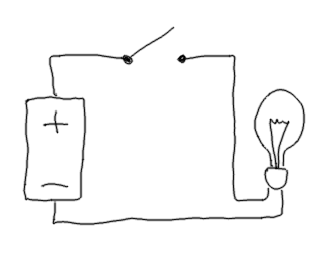
\includegraphics[height=1in]{pic/2.png}
\\
В этой цепи немного элементов: лампочка, батарея, ключ. Если ключ разомкнут,
ток не идёт, и лампочка не горит. Если ключ замкнут, ток идёт, и лампочка горит.
Кстати, лампочка нас интересует только как индикатор, есть ток или нет.
В целом зависимость ``лампочка - ключ'' можно охарактеризовать таблицей:
\\
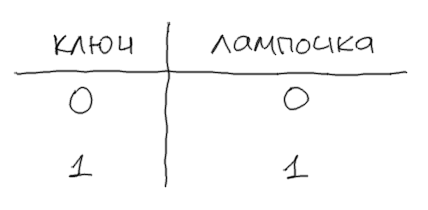
\includegraphics[height=1in]{pic/3.png}
\\
Таблицы такого рода, задающие зависимость истинности/ложности одних переменных
от истинности/ложности других переменных, называются \emph{таблицами истинности} или \emph{таблицами логики}.
Добавим ещё один ключ в схему (последовательно):
\\
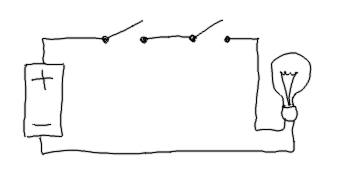
\includegraphics[height=1in]{pic/4.png}
\\
Теперь лампочка зависит от двух ключей: она горит, только если первый
\emph{и} второй ключ замкнут. Вот соответствующая таблица логики:
\\
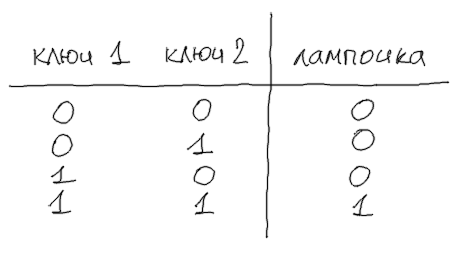
\includegraphics[height=1.5in]{pic/5.png}
\\
Если бы мы добавили второй ключ параллельно, схема бы получилась такой:
\\
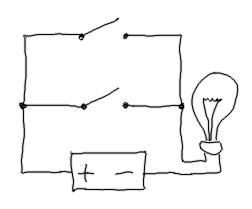
\includegraphics[height=1.5in]{pic/6.png}
\\
В этой схеме лампочка горит, только если первый \emph{или} второй ключ замкнут.
Вот её таблица логики:
\\
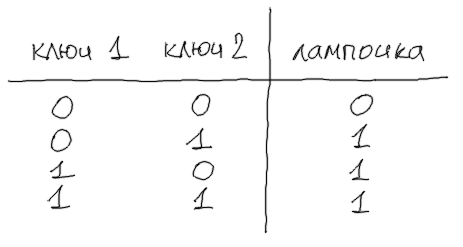
\includegraphics[height=1.5in]{pic/7.png}
\\
Мы получили две интересных схемы: первая отражает логическое \emph{и} (AND), вторая ---
логическое \emph{или} (OR). На основе этих схем можно собирать другие, более сложные.
Например, есть у тебя условие: ``если я сдам лабу или будет солнечно,
то я пойду гулять''. Это условие описывается схемой OR:
\\
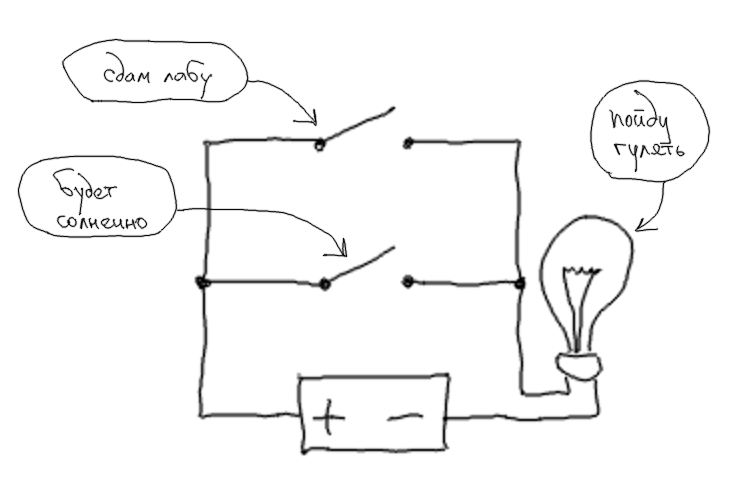
\includegraphics[height=2in]{pic/8.png}
\\
Преподаватель, которому ты собралась сдавать лабу, знает, что если у него
будет хорошее настроение, то ты сдашь лабу. Его настроение зависит от двух вещей:
во-первых, будет ли солнечно, а во вторых, успеет ли он пообедать.
Он может описать это с помощью схемы AND:
\\
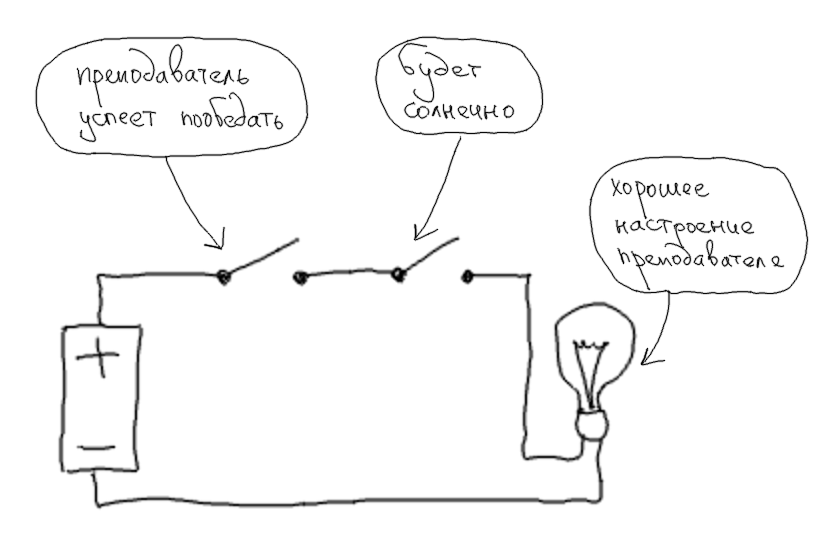
\includegraphics[height=2in]{pic/9.png}
\\
Допустим, преподаватель хочет узнать, пойдёшь ли ты завтра гулять, но не очень
хорошо разбирается в хитросплетениях твоей логики. Зато у него есть твоя схема.
Он берёт её и пытается присобачить к ней свою. Логически это очень просто:
нужно связать выход ``хорошее настроение'' со входом ``сдам лабу'': если на выходе
``хорошее настроение'' есть ток, ключ ``сдам лабу'' замкнут, если тока нет --
разомкнут:
\\
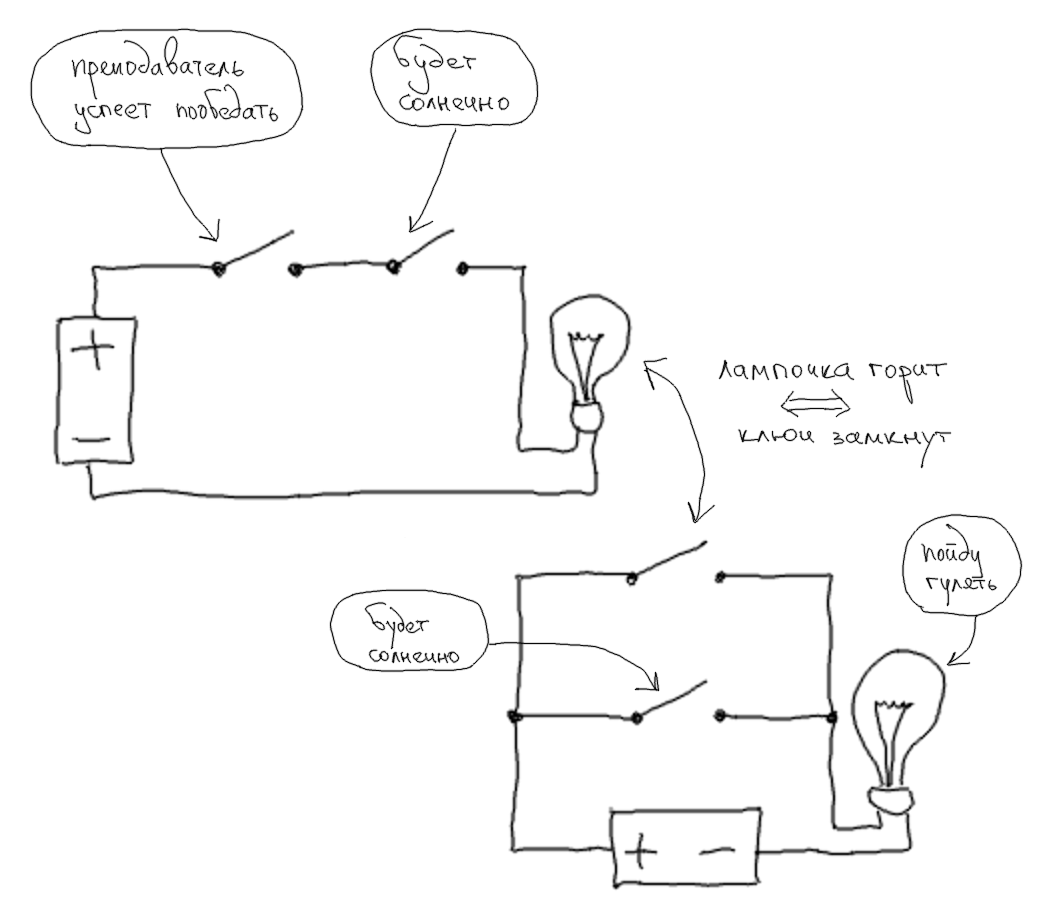
\includegraphics[height=3.5in]{pic/10.png}
\\
Поначалу можно вручную замыкать и размыкать ключ, но это быстро надоест
(особенно когда схема станет большой). Нужно что-то, что само замыкало и
размыкало бы ключ в зависимости от тока. Одним из таких устройств является
реле:
\\
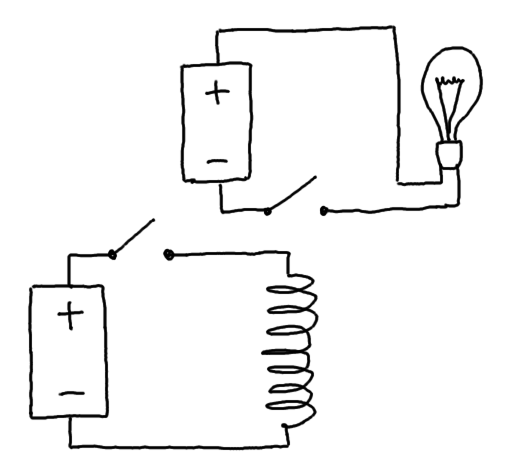
\includegraphics[height=2in]{pic/11.png}
\\
Если в первой цепи течёт ток, то катушка намагничивается и начинает притягивать
ключ во второй цепи. Ключ замыкается. Если в первой цепи ток пропадает, то катушка размагничивается,
перестаёт притягивать ключ и он размыкается. Реле позволяет связать вход
``сдам лабу'' с выходом ``хорошее настроение'':
\\
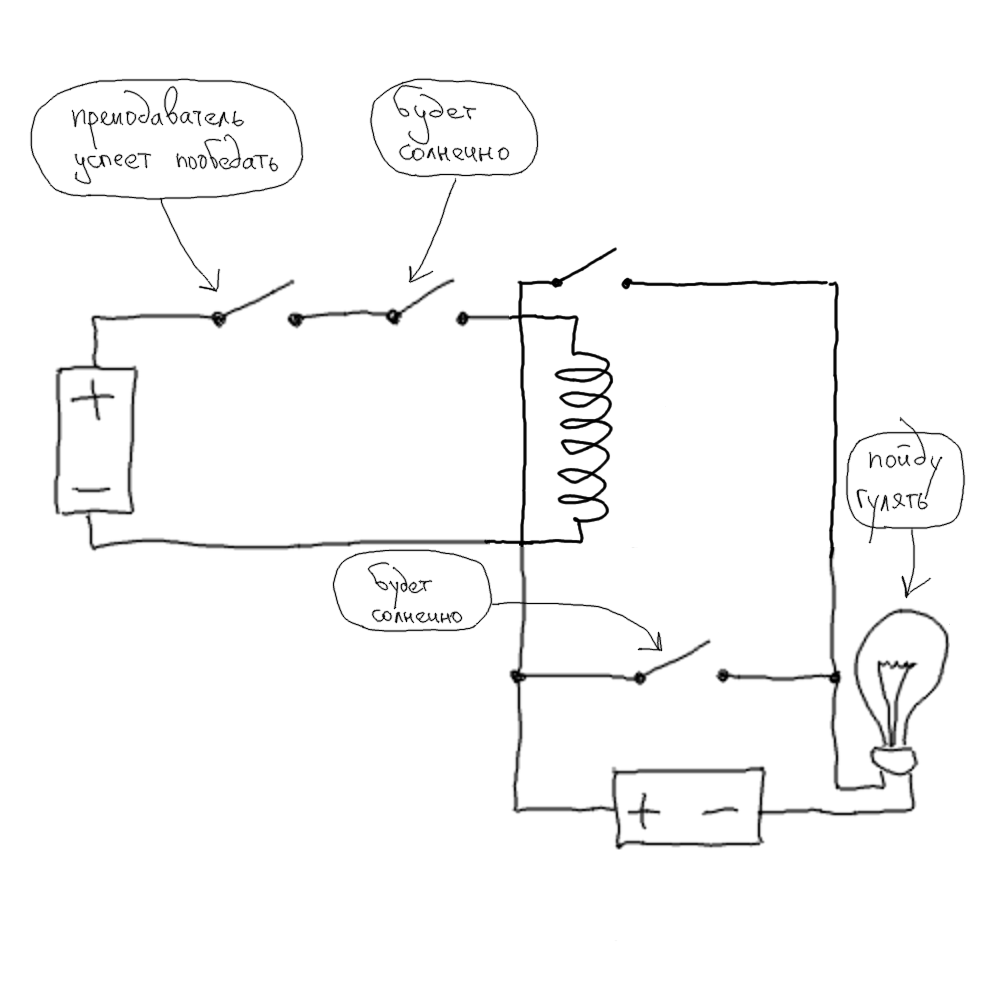
\includegraphics[height=3.5in]{pic/12.png}
\\
Конечно, эту конкретную схему можно упростить и выкинуть реле, просто встроив преподавательскую схему
в твою вместо ключа ``сдам лабу'':
\\
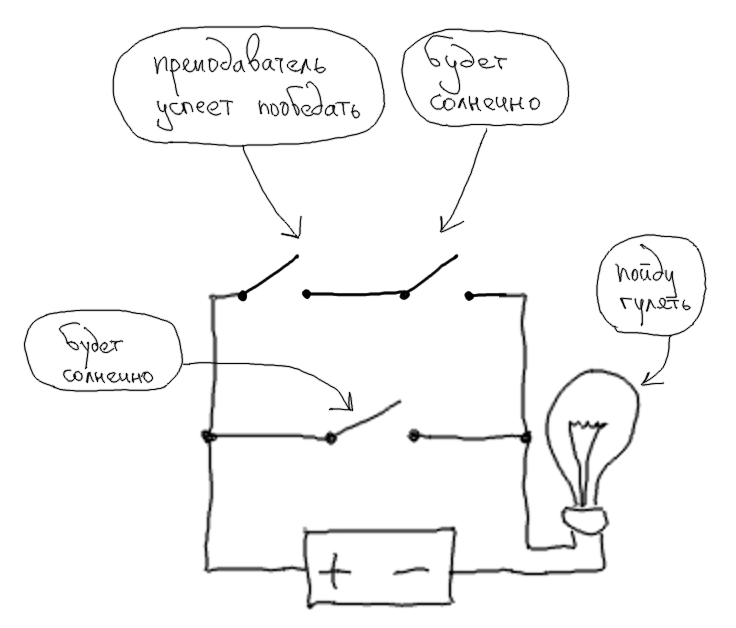
\includegraphics[height=3.5in]{pic/13.png}
\\
И даже ещё сильнее упростить:
\\
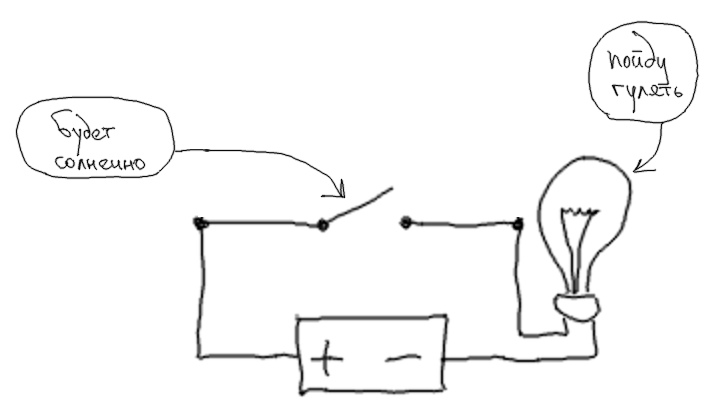
\includegraphics[height=2in]{pic/14.png}
\\
Но упростить не всегда возможно и никогда не поздно, и пусть этим занимаются разработчики микросхем.
Мне важно показать, что схему в принципе \emph{можно} собрать. Реле позволяет нам управлять входом схемы при помощи наличия/отсутствия тока,
а не при помощи замыкания/размыкания ключа. А наличие/отсутствие тока --- это как раз то,
что является выходом любой схемы. Поэтому можно сделать очень
важное предположение: что любой выход одной схемы можно соединить с любым входом другой
схемы. (Кстати, реле полезно не только для связывания разных схем, а ещё и просто как повторитель, для усиления слабого тока.
Именно для передачи сигнала на большие расстояния реле использовалось в телеграфных линиях.)
\\ \\
Реле --- не единственное устройство, способное замыкать и размыкать ключ
в зависимости от тока (но первое, которое применили в компьютерах). Сейчас
используются транзисторы, а до этого были вакуумные лампы.
\\ \\
Вот как выглядят схемы AND и OR с использованием реле:
\\
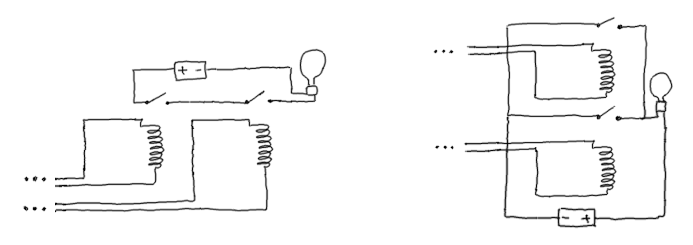
\includegraphics[height=2in]{pic/15.png}
\\
Строго говоря, это уже не схемы, а фрагменты схем. Но, с другой стороны, ``выход'' схемы ---
тоже не выход, а кусок цепи, по которому идёт или не идёт ток. Чтобы соединить выход
и фрагмент, нужно разомкнуть цепь в районе выхода и получившиеся два конца провода примотать
к концам провода, торчащим из фрагмента:
\\
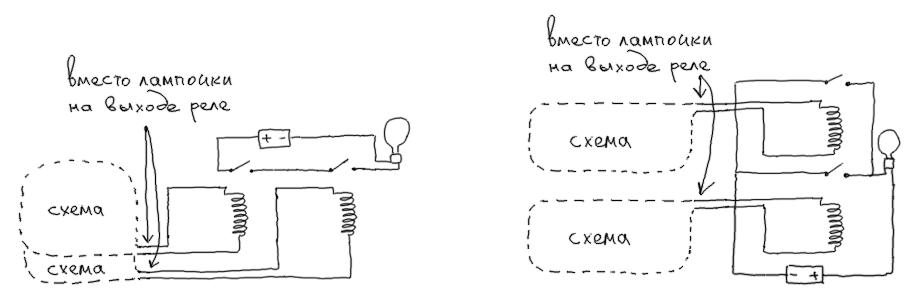
\includegraphics[height=2in]{pic/16.png}
\\
Дальше я всё буду называть схемой. Вот ещё одна важная схема, отражающая ``логическое \emph{не}'', NOT:
\\
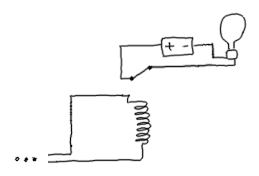
\includegraphics[height=1.5in]{pic/17.png}
\\
В предыдущих схемах реле повторяло сигнал, а здесь оно его инвертирует: если в первой цепи идёт ток, то во второй тока нет, и наоборот.
Поэтому схема называется \emph{инвертором}.
\\ \\
Оказывается, что вместе три эти простенькие схемы --- И, ИЛИ, НЕ --- обладают невероятной силой.
С помощью них можно собрать ЛЮБУЮ логическую схему! (И это ещё не всё: из схем И и НЕ можно
собрать схему ИЛИ, а из схем ИЛИ и НЕ можно собрать схему И. Есть вообще такие схемы И-НЕ и ИЛИ-НЕ,
что с помощью каждой из них (одной) можно собрать все остальные. Дальше по этой
теме читай про ``полные системы булевых функций''.)
\\ \\
Для этих трёх схем --- И, ИЛИ, НЕ --- я введу общепринятые обозначения:
\\ \\
Как видишь, входы и выходы обозначаются одинаково, в виде куска торчащего
провода. Я буду говорить ``подать ток на вход''. Понятно, что с точки зрения физики это
бред, потому что нельзя просто так взять и подать ток куда-то. Но (надеюсь) понятно,
что я имею в виду.
\\ \\
Почти всё дальнейшее построение компьютера сведётся к сборке более сложных схем
из этих трёх.

\subsection{Двоичная система счисления}
Я вот всё время говорю про логические схемы и булевые функции (что по сути одно и то же),
и даже собрала маленькую схему для определения, пойдёшь ли ты гулять. Более того, я собрала
несколько простых схем (И, ИЛИ, НЕ) и говорю, что с их помощью можно собрать
любую логическую схему. В смысле логических схем наще будущее явно обеспечено.
Но всё-таки, какая ИМЕННО от них польза?
\\ \\
Пока понятно только, что электричество удивительно хорошо для них подходит.
В электричестве есть два чётких состояния: есть ток, нет тока. И в логике
есть два элемента: правда, ложь. Если б мы захотели с помощью электричества моделировать
социальные анкеты (``да'', ``нет'', ``не знаю''), нам пришлось бы выдумывать, как обозначать
третий элемент (например, есть ток, но слабый). Тем более тяжело было бы
с десятичными цифрами.
\\ \\
А мы-то как раз с цифрами (вернее, с числами) работать и собрались, потому что
что это за компьютер, который даже два числа сложить не может. К счастью, нам не
придётся моделировать десять состояний (в отличие от тех, кто строил первые
компьютеры). Мы просто будем все вычисления внутри компьютера проводить над числами
в двоичном представлении.
\\ \\
Важное замечание: от того, что мы решили использовать в компьютере двоичные,
а не десятичные числа, С ТОЧКИ ЗРЕНИЯ ПОЛЬЗОВАТЕЛЯ НИЧЕГО НЕ МЕНЯЕТСЯ: число
это просто абстрактная идея, и не важно, в каком виде она выражена. Компьютер
будет делать ровно то же, что и с десятичными числами: решать такие же задачи
и выдавать такие же результаты. Потом, если угодно, можно сделать специальную приставку,
которая будет позволять вводить/выводить десятичные числа, и переводить их
для компьютера в двоичное представление.

\section{Сумматор}
Итак, компьютер нужен для автоматизации вычислений.
Поэтому первое, без чего не обойдётся ни один компьютер, это устройство
для сложения чисел. Попробуем собрать такое устройство --- сумматор.
\\ \\
Чтобы понять, как должен работать двоичный сумматор, надо
вспомнить, что делает человек, когда складывает двоичные числа.
Сложение происходит поразрядно и с переносом:

\begin{enumerate}
\item
   k = 1
\\
   перенос = 0
\\
   если одно число короче другого, дополнить его нулями в старших разрядах
\\
   N = число разрядов
\\
\item Определяем k-й разряд первого суммы и новый перенос по таблице:
\begin{verbatim}
   -------------------------------------------------------------------
   | k-й разряд    | k-й разряд    | перенос || k-й разряд | перенос |
   | первого числа | второго числа |         || суммы      | (новый) |
   |---------------|---------------|---------||------------|---------|
   |       0       |       0       |    0    ||     0      |    0    |
   |       0       |       0       |    1    ||     1      |    0    |
   |       0       |       1       |    0    ||     1      |    0    |
   |       0       |       1       |    1    ||     0      |    1    |
   |       1       |       0       |    0    ||     1      |    0    |
   |       1       |       0       |    1    ||     0      |    1    |
   |       1       |       1       |    0    ||     0      |    1    |
   |       1       |       1       |    1    ||     1      |    1    |
   -------------------------------------------------------------------
\end{verbatim}
\item k = k + 1
\item если k < N
\\
       перейти к шагу 2
\end{enumerate}


Видимо, главное в этом алгортме --- таблица, по которой определяются новый перенос
и k-й разряд суммы. Без этой таблицы не обойтись: в жизни мы принимаем как аксиому,
что 0+0=0, 0+1=1, 1+0=1, 1+1=0 и 1 в уме. В сумматор тоже придётся встроить эти
правила.
\\ \\
Итак, нам нужна схема, у которой три входа: k-й разряд первого слагаемого,
k-й разряд второго слагаемого и перенос, и два выхода: k-й разряд суммы и перенос
на (k + 1)-й разряд. Отстуствие тока на входе или выходе означает ноль,
наличие --- единицу. Внутри схема должна быть устроена так, чтобы зависимость
выходов от входов была такая же, как в таблице.
\\ \\
Это очень похоже на схемы И, ИЛИ, НЕ, только наша схема более сложная.
Чтобы слегка упростить схему, разобьём её на две полсхемы. Сделать это
можно так: вместо того, чтобы сразу пытаться сложить три входа
(k-й разряд первого числа, k-й разряд второго числа, перенос), будем
два раза складывать по два входа: сначала k-й разряд первого числа и k-й разряд второго числа,
а потом результат первого сложения и перенос.
\\ \\
Когда складываешь два входа, может возникнуть перенос (если оба входа равны 1).
Поэтому у каждой полсхемы будет два входа (для слагаемых) и два выхода
(для суммы и переноса):
\begin{verbatim}
   ----------------------------------------------------
   | 1-е слагаемое | 2-е слагаемое || сумма | перенос |
   |               |               ||       |         |
   |---------------|---------------||-------|---------|
   |       0       |       0       ||     0 |     0   |
   |       0       |       1       ||     1 |     0   |
   |       1       |       0       ||     1 |     0   |
   |       1       |       1       ||     0 |     1   |
   ----------------------------------------------------
\end{verbatim}
Чтобы собрать такую полсхему, снова разобьём её на две четвертьсхемы,
одна для суммы, а вторая для переноса:
\begin{verbatim}
   ------------------------------------------
   | 1-е слагаемое | 2-е слагаемое || сумма |
   |               |               ||       |
   |---------------|---------------||-------|
   |       0       |       0       ||     0 |
   |       0       |       1       ||     1 |
   |       1       |       0       ||     1 |
   |       1       |       1       ||     0 |
   ------------------------------------------
   --------------------------------------------
   | 1-е слагаемое | 2-е слагаемое || перенос |
   |               |               ||         |
   |---------------|---------------||---------|
   |       0       |       0       ||     0   |
   |       0       |       1       ||     0   |
   |       1       |       0       ||     0   |
   |       1       |       1       ||     1   |
   --------------------------------------------
\end{verbatim}

Четвертьсхема для переноса совсем простая --- это попросту схема И.
С суммой всё не так просто, но взяв две схемы ИЛИ, одну схему НЕ и одну схему И,
мы получим то, что надо:
\\ \\
Остаётся объединить входы четвертьсхем для суммы и переноса,
и полсхема для сложения двух входов готова:
\\ \\
Теперь пора связать полсхемы. У первой полсхемы два входа:
k-й разряд первого слагаемого и k-й разряд второго слагаемого.
У второй полсхемы первый вход --- это выход ``сумма'' первой полсхемы,
а второй вход --- перенос:
\\ \\
У нас остался один выход ``сумма'' --- как раз как надо. Но выходов ``перенос'' по прежнему два,
а нужен один. Из-за разбиения сложения на два этапа на каждом этапе получился свой перенос.
Но ведь в жизни всё равно, сразу три числа складывать, или сначала сложить два, а потом прибавить
третье --- результат один и тот же. Что-то тут не то! Если повнимательнее рассмотреть полученную нами схему
с тремя выходами, то её работа описывается такой таблицей логики:
\begin{verbatim}
   -------------------------------------------------------------------------------------
   | k-й разряд    | k-й разряд    | перенос || k-й разряд | 1-й перенос | 2-й перенос |
   | первого числа | второго числа |         || суммы      |             |             |
   |---------------|---------------|---------||------------|-------------|-------------|
   |       0       |       0       |    0    ||     0      |    0        |    0        |
   |       0       |       0       |    1    ||     1      |    0        |    0        |
   |       0       |       1       |    0    ||     1      |    0        |    0        |
   |       0       |       1       |    1    ||     0      |    0        |    1        |
   |       1       |       0       |    0    ||     1      |    0        |    0        |
   |       1       |       0       |    1    ||     0      |    0        |    1        |
   |       1       |       1       |    0    ||     0      |    1        |    0        |
   |       1       |       1       |    1    ||     1      |    1        |    0        |
   -------------------------------------------------------------------------------------
\end{verbatim}

Из таблицы видно, что хотя переноса два, они не бывают одновременно равны 1.
Поэтому их можно объединить при помощи схемы ИЛИ:
\\ \\
Готово! Вот она, чудо-схема для сложения разрядов с переносом.

\section{Команды}
...
\section{Память}
...
\section{Счётчик}
...
\chapter{Переход к языкам высокого уровня}
...
\section{Ассемблер}
...
\section{Необходимость абстрагироваться от машины}
...
\section{Языковые процессоры}
...
\subsection{Компиляторы}
...
\subsection{Интерпретаторы}
...
\subsection{JIT-компиляторы}
...
\subsection{Промежуточные представления}
...
\subsection{Виртуальные машины}
...
\subsection{Детсадовский пример}
\definecolor{cgray}{rgb}{0.96, 0.95, 0.9}
\definecolor{cblue1}{rgb}{0.0, 0.15, 0.3}
\definecolor{cblue2}{rgb}{0.0, 0.4, 0.6}
\definecolor{cblue3}{rgb}{0.0, 0.7, 1.0}
\definecolor{cgreen}{rgb}{0.2, 0.6, 0.0}
\lstdefinestyle{cxx}
    { numbers=left
    , numberstyle=\footnotesize\ttfamily\color{cblue3}
    , breaklines=true
    , language=C++
    , basicstyle=\footnotesize\ttfamily\color{cblue1}
    , keywordstyle=\footnotesize\ttfamily\color{cblue2}
    , commentstyle=\itshape\color{cgreen}
    , backgroundcolor=\color{cgray}
    }
\lstset{style=cxx}
...
\subsubsection{Язык}
...
\subsubsection{Парсер}
\lstinputlisting[language=C++]{example_lang_proc/parser.cpp}
\lstinputlisting[language=C++]{example_lang_proc/parser.h}
\subsubsection{Интерпретатор}
\lstinputlisting[language=C++]{example_lang_proc/interpreter.cpp}
\lstinputlisting[language=C++]{example_lang_proc/interpreter.h}
\subsubsection{Компилятор}
\lstinputlisting[language=C++]{example_lang_proc/compiler.cpp}
\lstinputlisting[language=C++]{example_lang_proc/compiler.h}
\subsubsection{Виртуальная машина: байткод}
\lstinputlisting[language=C++]{example_lang_proc/vm_bytecode.cpp}
\lstinputlisting[language=C++]{example_lang_proc/vm_bytecode.h}
\subsubsection{Виртуальная машина: интерпретатор байткода}
\lstinputlisting[language=C++]{example_lang_proc/vm_run.cpp}
\lstinputlisting[language=C++]{example_lang_proc/vm_run.h}
\subsubsection{Виртуальная машина: JIT-компилятор байткода}
\lstinputlisting[language=C++]{example_lang_proc/vm_jit.cpp}
\lstinputlisting[language=C++]{example_lang_proc/vm_jit.h}
\subsection{Как всё в реальной жизни}
...
\section{Синтаксический анализ}
...
\chapter{Основы языков программирования}
...
\section{Синтаксис и семантика}
...
\section{Структура языка}
...
\subsection{Примитивы}
...
\subsection{Переменные}
...
\subsection{Типы}
...
\subsection{Выражения}
...
\subsection{Утверждения}
...
\subsection{Управляющие конструкции}
...
\subsection{Функции}
...
\subsection{Сложные типы и отношения между типами}
...
\subsection{Области видимости}
...
\subsection{Полиморфизм (параметрический, ad-hoc, полиморфизм подтипов)}
...
\subsection{Расширяемость}
...
\section{Язык в действии}
...
\subsection{Выразительная сила языка (тьюринг-полнота)}
...
\subsection{Математическая модель вычислений}
...
\subsection{Статическое и динамическое в языке}
...
\subsection{Управление памятью}
...
\subsection{Параллельные вычисления}
...
\subsection{Динамическая генерация кода}
...
\subsection{Рантайм и стандартная библиотека}
...
\section{Что важно для программиста}
...

\end{document}